% =========================
% CHƯƠNG 5
% =========================
\chapter{Điều khiển pha thích nghi (APC)}

\section{Nguyên lý thiết kế và kiến trúc}

Bộ điều khiển pha thích nghi (Adaptive Phase Controller - APC) được thiết kế theo nguyên lý điều khiển phân tán với khả năng tự quyết định cục bộ cho từng nút giao thông. Kiến trúc này cho phép mỗi nút giao hoạt động độc lập trong khi vẫn có thể phối hợp với các nút lân cận thông qua cơ chế trao đổi thông tin. APC kết hợp giữa điều khiển dựa trên luật (rule-based control) để đảm bảo an toàn và điều khiển thích ứng (adaptive control) để tối ưu hiệu suất.

\begin{figure}[H]
    \centering
    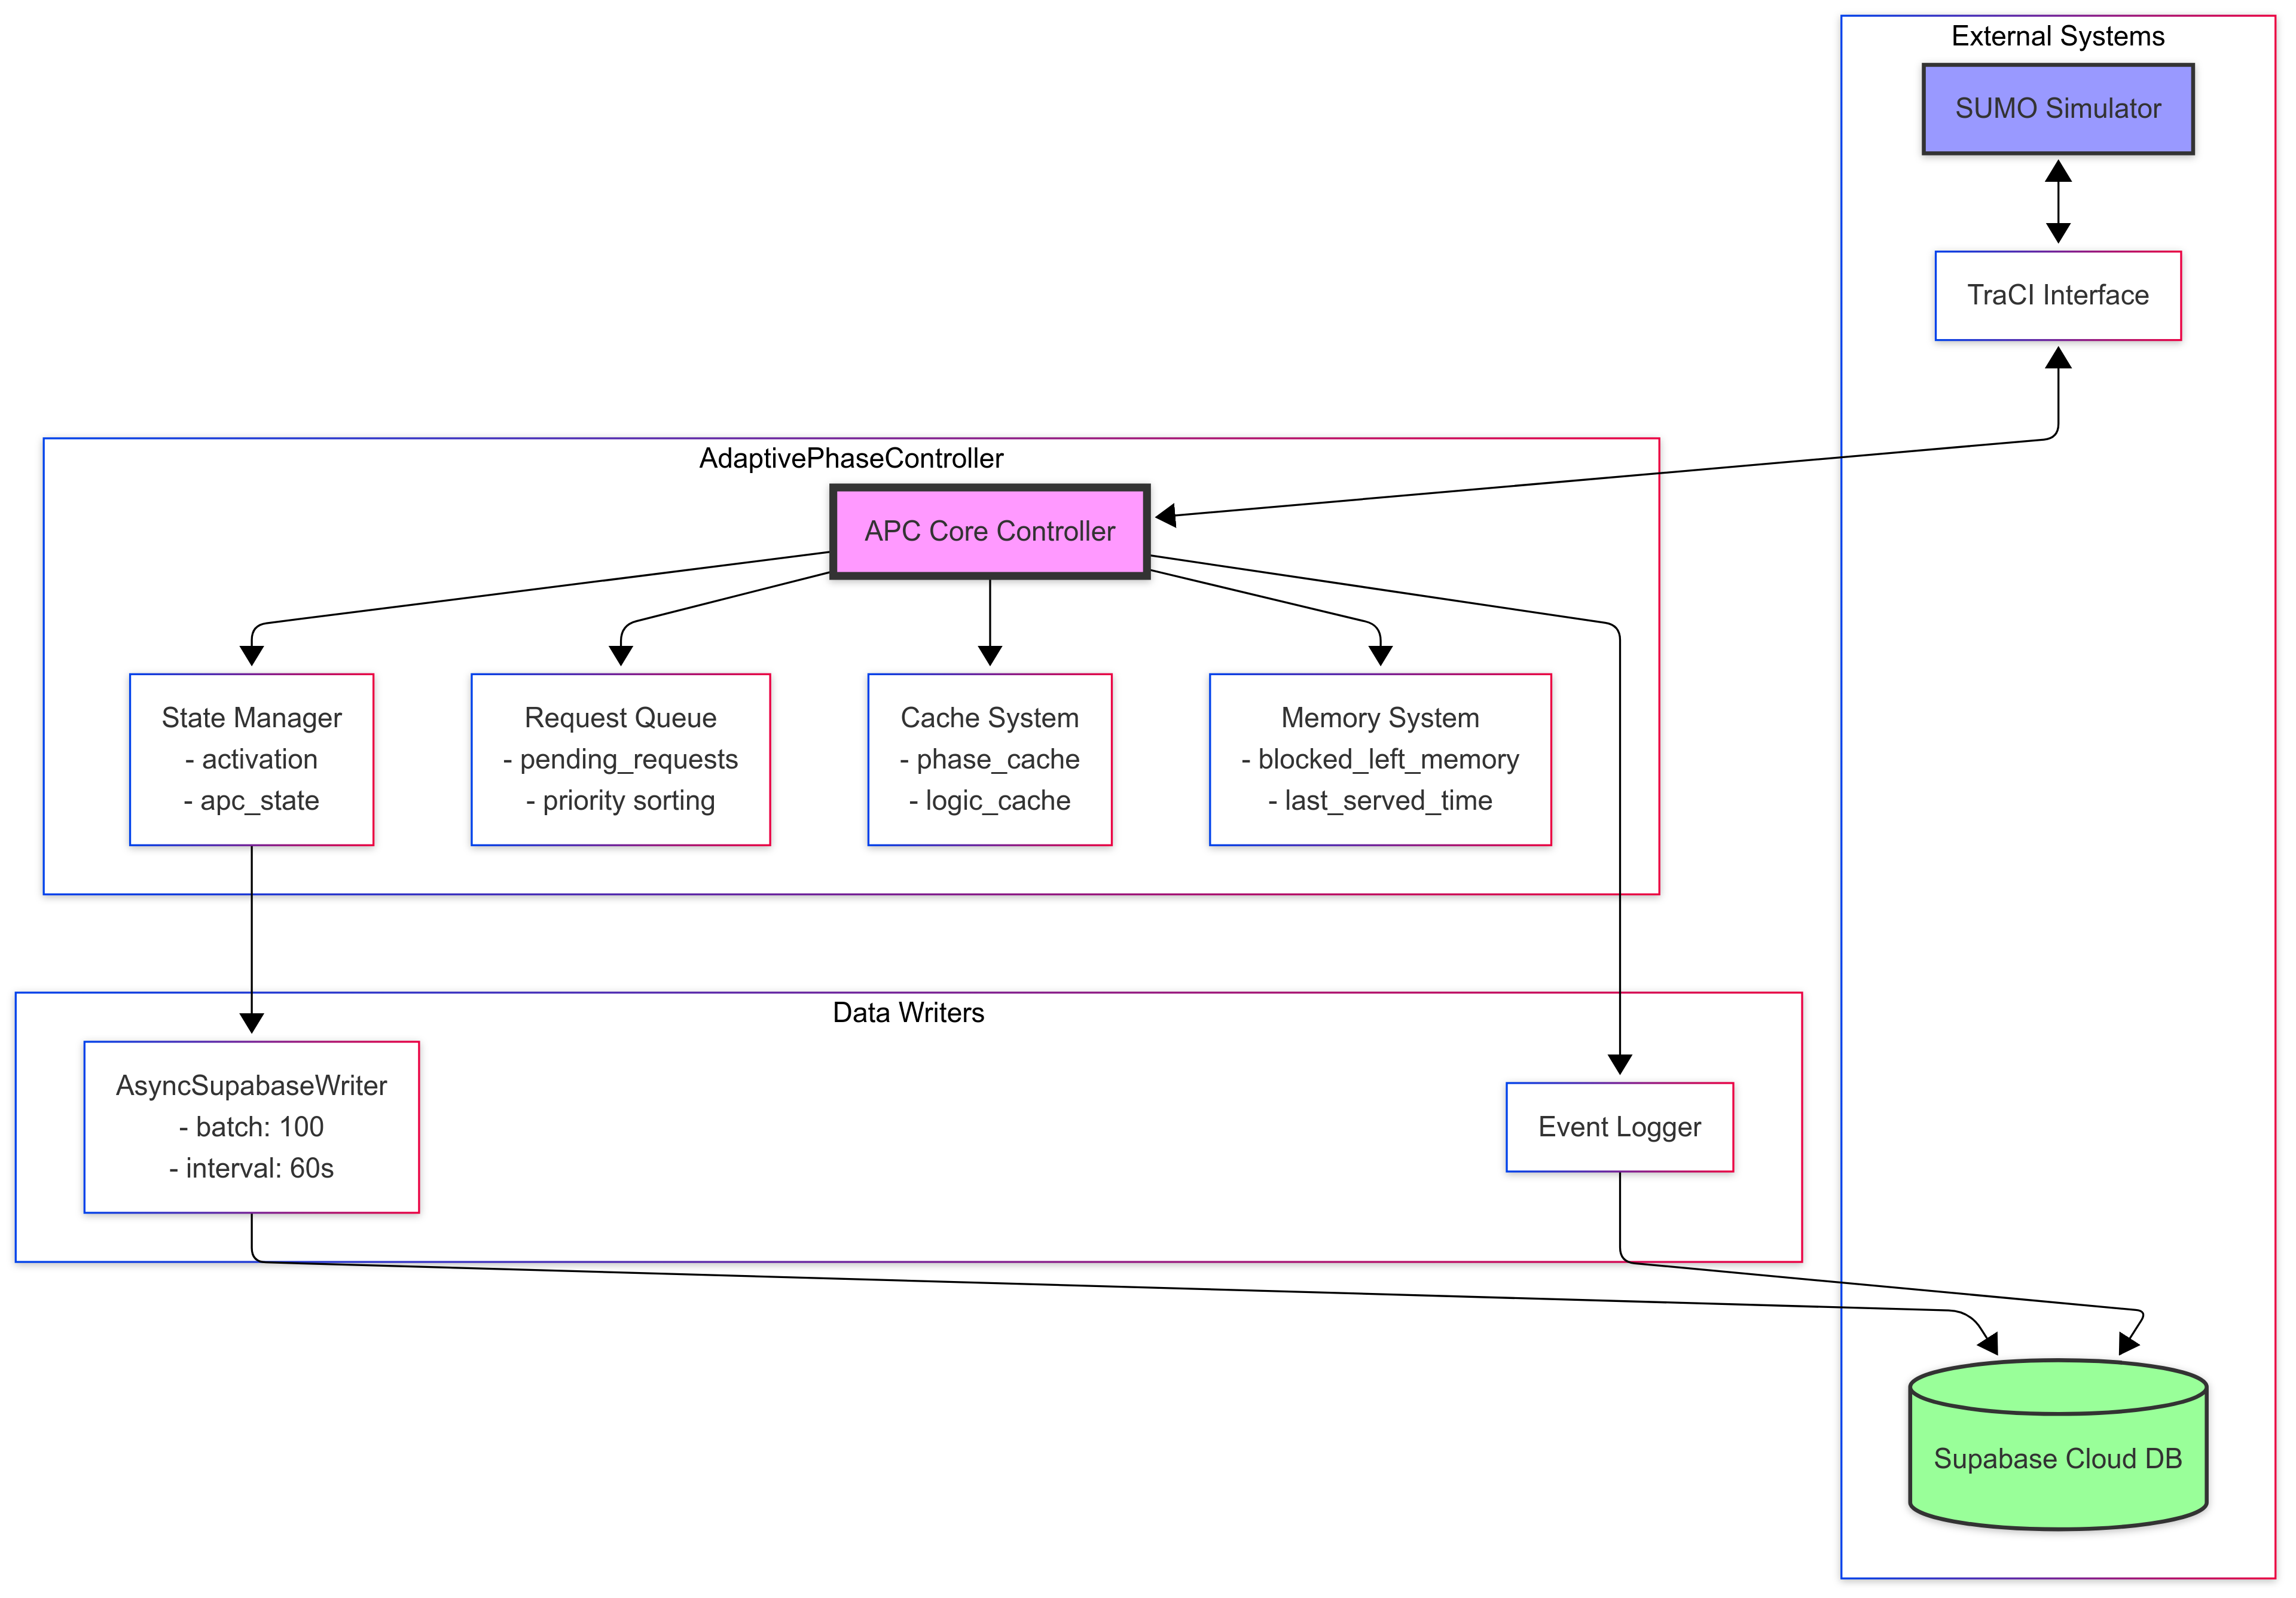
\includegraphics[width=0.9\textwidth]{Untitled diagram _ Mermaid Chart-2025-08-21-074754.png}
    \caption{Kiến trúc tổng thể của bộ điều khiển APC với các thành phần chính và luồng dữ liệu}
    \label{fig:apc_architecture}
\end{figure}

\subsection{Khởi tạo và cấu hình hệ thống}

Quá trình khởi tạo APC được thực hiện qua constructor với các tham số quan trọng:

\begin{lstlisting}[style=py, caption={Khởi tạo AdaptivePhaseController}]
def __init__(self, lane_ids, tls_id, alpha=1.0, 
             min_green=30, max_green=80,
             r_base=0.5, r_adjust=0.1, 
             severe_congestion_threshold=0.8,
             large_delta_t=20):
    self.lane_ids = lane_ids
    self.tls_id = tls_id
    # Đăng ký subscription với TraCI
    for lid in self.lane_ids:
        traci.lane.subscribe(lid, [
            traci.constants.LAST_STEP_VEHICLE_HALTING_NUMBER,
            traci.constants.LAST_STEP_MEAN_SPEED,
            traci.constants.LAST_STEP_VEHICLE_NUMBER,
            traci.constants.LAST_STEP_VEHICLE_ID_LIST,
        ])
\end{lstlisting}

\textbf{Quá trình khởi tạo bao gồm các bước chính:}

\begin{enumerate}
    \item \textbf{Thiết lập subscription với TraCI:} Hệ thống đăng ký theo dõi các metrics quan trọng cho từng làn đường được quản lý, bao gồm số lượng xe dừng, tốc độ trung bình, tổng số xe và danh sách ID phương tiện. Cơ chế subscription giúp tối ưu băng thông bằng cách chỉ nhận dữ liệu cần thiết.
    
    \item \textbf{Khởi tạo cấu trúc dữ liệu:} Các container quan trọng được khởi tạo:
    \begin{itemize}
        \item \texttt{apc\_state}: Dictionary lưu trữ trạng thái toàn cục với events queue (maxlen=5000) và danh sách phases
        \item \texttt{pending\_requests}: Hàng đợi yêu cầu chuyển pha với cơ chế ưu tiên
        \item \texttt{phase\_cache}: Cache thông tin pha với TTL 30 giây để giảm truy vấn database
        \item \texttt{blocked\_left\_memory}: Dictionary theo dõi lịch sử làn rẽ trái bị chặn
    \end{itemize}
    
    \item \textbf{Kết nối database:} Khởi tạo \texttt{PatchedAsyncSupabaseWriter} với interval 60 giây và batch size 100 records để đồng bộ dữ liệu không đồng bộ lên cloud.
    
    \item \textbf{Tải trạng thái từ Supabase:} Phương thức \texttt{\_load\_apc\_state\_supabase()} được gọi để khôi phục trạng thái từ lần chạy trước, đảm bảo tính liên tục của hệ thống.
    
    \item \textbf{Đồng bộ pha với SUMO:} \texttt{preload\_phases\_from\_sumo()} đảm bảo tất cả các pha trong logic đèn được ghi nhận và có base duration phù hợp.
\end{enumerate}
\begin{figure}[H]
    \centering
    \begin{subfigure}[b]{0.65\textwidth}
        \centering
        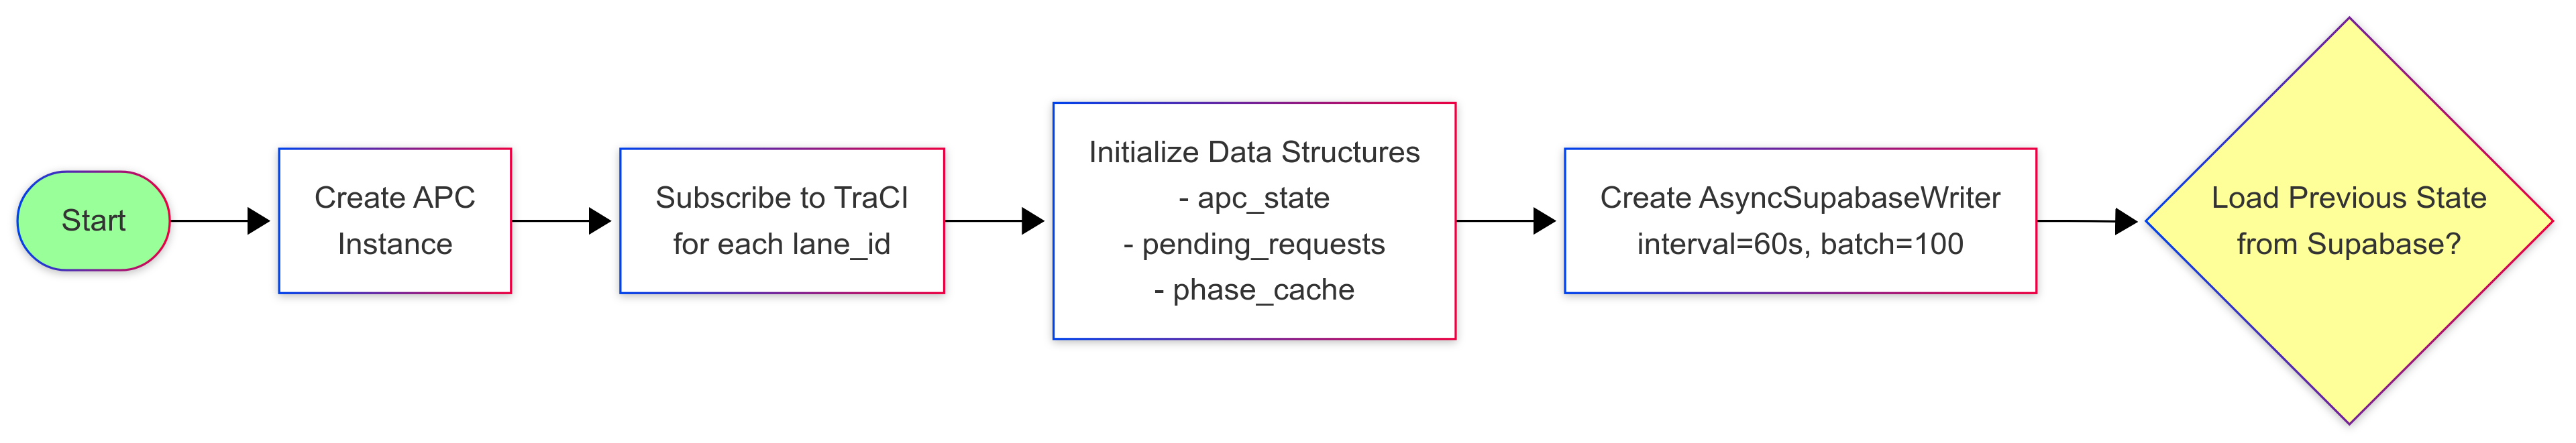
\includegraphics[width=\textwidth]{Untitled diagram _ Mermaid Chart-2025-08-21-084042.png}
        \caption{Khởi tạo và thiết lập}
    \end{subfigure}
    \hfill
    \begin{subfigure}[b]{0.65\textwidth}
        \centering
        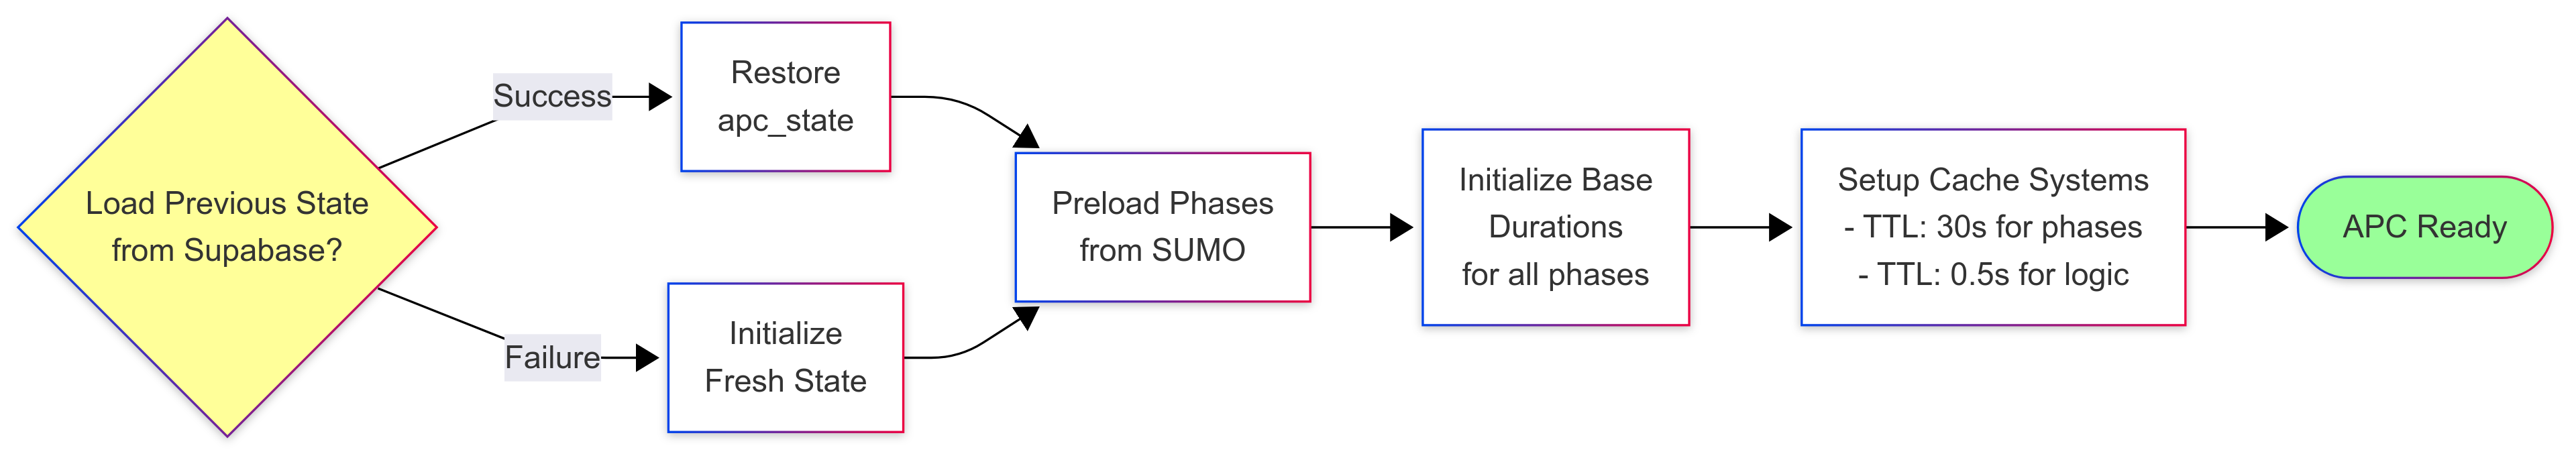
\includegraphics[width=\textwidth]{Untitled diagram _ Mermaid Chart-2025-08-21-084132.png}
        \caption{Khôi phục trạng thái và hoàn tất}
    \end{subfigure}
    \caption{Quy trình khởi tạo AdaptivePhaseController. \newline \textbf{Lưu ý:} Đã tăng kích thước hình để dễ quan sát hơn.}
    \label{fig:apc_init_flow}
\end{figure}
\subsection{Cấu trúc dữ liệu và tham số điều khiển}

APC sử dụng hệ thống tham số phân cấp để điều chỉnh hành vi:

\subsubsection{Tham số thời gian}
\begin{itemize}
    \item \texttt{min\_green} (mặc định 30s): Thời gian tối thiểu cho mỗi pha xanh, đảm bảo an toàn và công bằng
    \item \texttt{max\_green} (mặc định 80s): Giới hạn trên để tránh monopoly một hướng
    \item \texttt{cycle\_length} (mặc định 90s): Chu kỳ tham chiếu cho điều phối corridor
    \item \texttt{low\_demand\_extend\_cap} (4s): Giới hạn mở rộng khi nhu cầu thấp
\end{itemize}

\subsubsection{Tham số điều khiển thích ứng}
\begin{itemize}
    \item \texttt{alpha} (1.0): Hệ số học trong công thức điều chỉnh $\Delta t = \alpha(R - R_{target})$
    \item \texttt{r\_base} (0.5): Giá trị reward cơ sở cho thuật toán học
    \item \texttt{r\_adjust} (0.1): Hệ số điều chỉnh R\_target động
    \item \texttt{weights} (vector 4D): Trọng số cho [density, speed, wait, queue] trong hàm reward
\end{itemize}

\subsubsection{Ngưỡng phát hiện sự kiện}
\begin{itemize}
    \item \texttt{severe\_congestion\_threshold} (0.8): Tỷ lệ queue/capacity kích hoạt chế độ khẩn cấp
    \item \texttt{protected\_left\_min\_queue} (5): Số xe tối thiểu để kích hoạt rẽ trái bảo vệ
    \item \texttt{min\_starve\_queue} (2): Ngưỡng phát hiện starvation
    \item \texttt{hysteresis\_margin} (0.10): Yêu cầu cải thiện 10\% để chuyển pha
\end{itemize}
\begin{figure}[H]
    \centering
    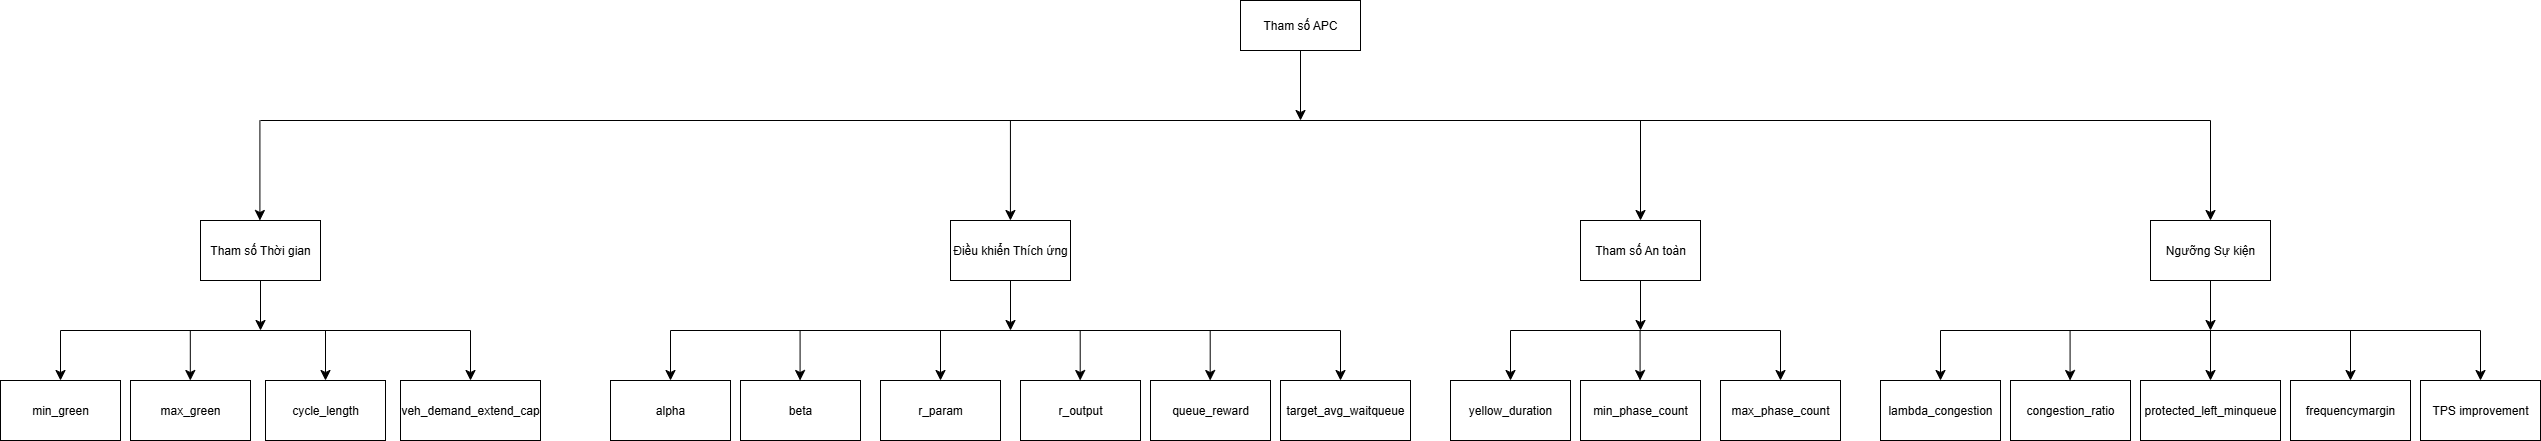
\includegraphics[width=1.1\textwidth]{Untitled Diagram.drawio (8).png}
    \caption{Phân cấp tham số điều khiển trong APC}
    \label{fig:parameter_hierarchy}
\end{figure}
\subsubsection{Cấu trúc dữ liệu chính}

\textbf{Activation State:} Dictionary theo dõi pha đang hoạt động:
\begin{lstlisting}[style=py]
self.activation = {
    "phase_idx": None,        # Chi so pha hien tai
    "start_time": 0.0,        # Thoi diem bat dau
    "base_duration": None,    # Thoi luong co so
    "desired_total": None     # Thoi luong mong muon
}
\end{lstlisting}

\textbf{Pending Requests Queue:} Danh sách các yêu cầu chuyển pha được sắp xếp theo priority và timestamp:
\begin{lstlisting}[style=py]
request = {
    "phase_idx": int,         # Pha muc tieu
    "priority": int,          # Muc uu tien (1-11)
    "priority_type": str,     # Loai: emergency, starvation...
    "extension_duration": float,  # Thoi luong yeu cau
    "timestamp": float        # Thoi diem tao yeu cau
}
\end{lstlisting}
\begin{figure}[H]
    \centering
    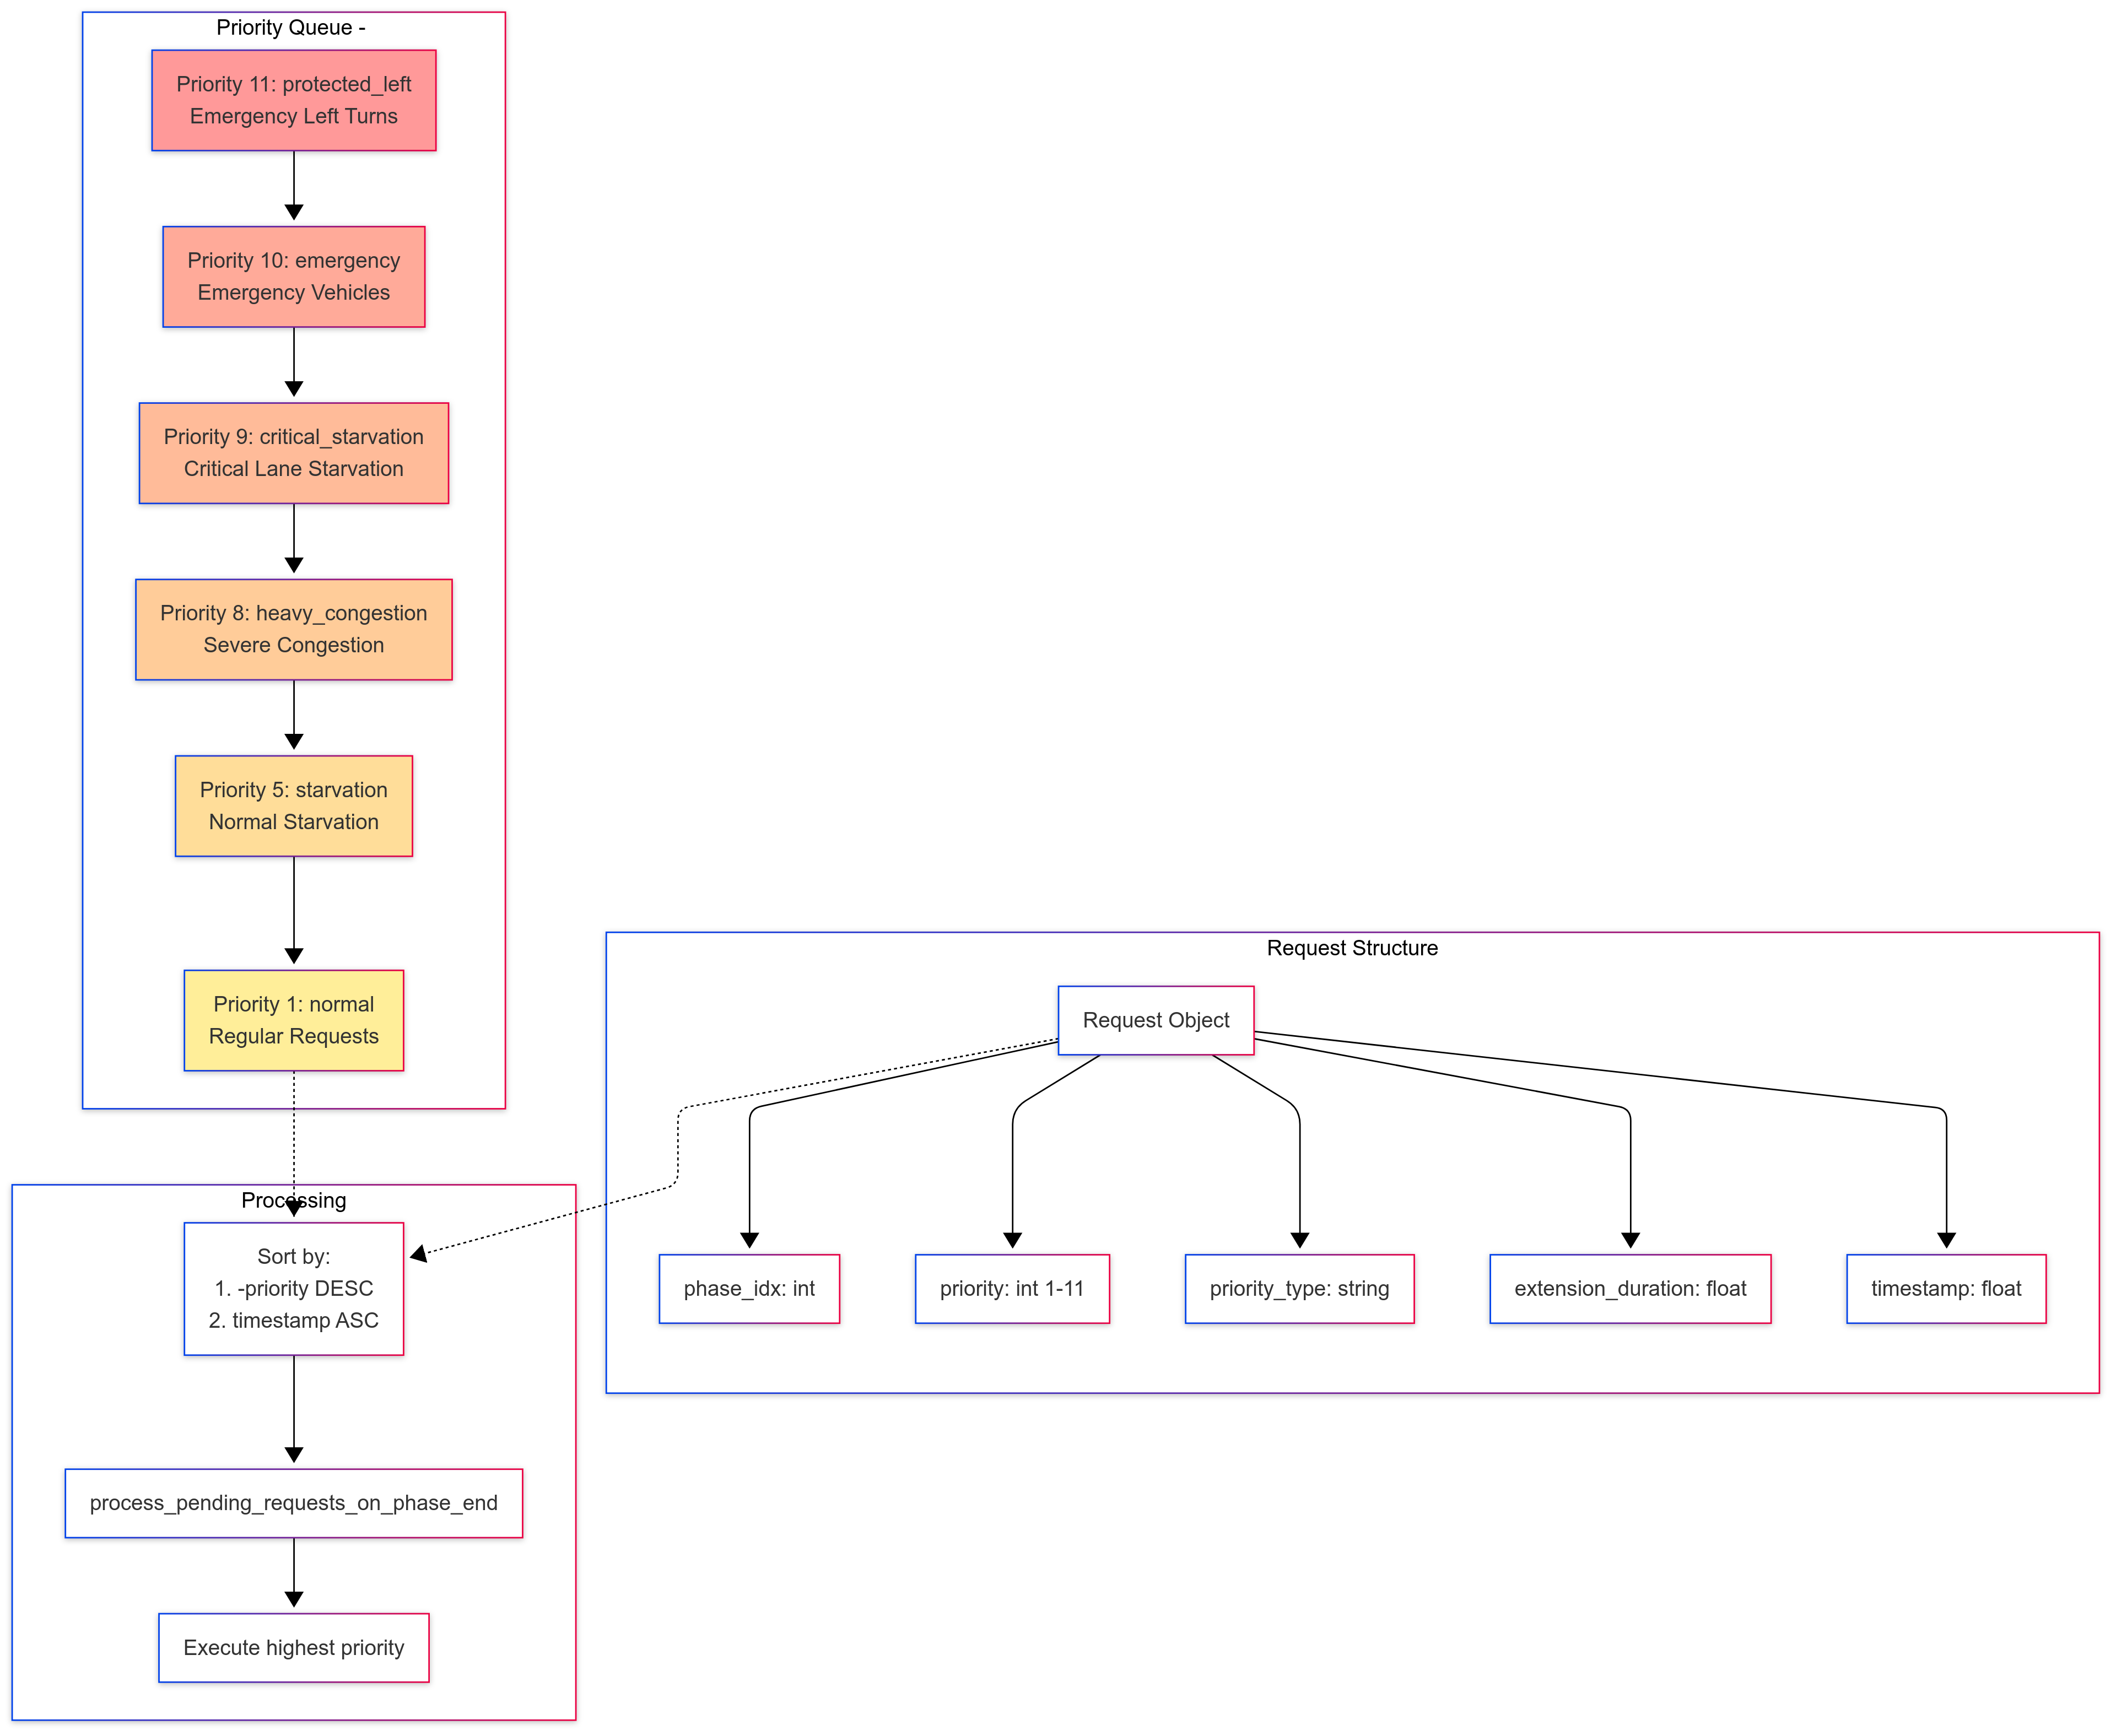
\includegraphics[width=0.75\textwidth]{Untitled diagram _ Mermaid Chart-2025-08-22-023041.png}
    \caption{Cấu trúc hàng đợi yêu cầu với mức độ ưu tiên}
    \label{fig:priority_queue}
\end{figure}
\subsection{Tích hợp với TraCI và SUMO}

Việc tích hợp với SUMO thông qua TraCI được thực hiện qua nhiều lớp abstraction:

\subsubsection{Subscription Mechanism}
APC sử dụng TraCI subscription để nhận dữ liệu real-time hiệu quả:

\begin{lstlisting}[style=py, caption={Xử lý subscription results}]
def get_lane_stats(self, lane_id):
    res = traci.lane.getSubscriptionResults(lane_id) or {}
    q = float(res.get(
        traci.constants.LAST_STEP_VEHICLE_HALTING_NUMBER,
        traci.lane.getLastStepHaltingNumber(lane_id)
    ))
    v = float(res.get(
        traci.constants.LAST_STEP_MEAN_SPEED,
        traci.lane.getLastStepMeanSpeed(lane_id)
    ))
    return q, w, v, dens
\end{lstlisting}

\subsubsection{Logic Cache System}
Để giảm overhead communication, APC implement cache cho traffic light logic:

\begin{lstlisting}[style=py, caption={Cơ chế cache logic}]
def _get_logic(self):
    now = traci.simulation.getTime()
    if self._logic_cache is None or \
       now - self._logic_cache_at > self._logic_cache_ttl:
        self._logic_cache = get_current_logic(self.tls_id)
        self._logic_cache_at = now
    return self._logic_cache
\end{lstlisting}

Cache có TTL 0.5 giây và được invalidate khi có thay đổi cấu trúc pha. Hệ thống còn hỗ trợ shared cache ở controller level để tối ưu cho nhiều APC instances.

\subsubsection{Safe Control Wrappers}
Mọi lệnh điều khiển được wrap trong các hàm an toàn:

\begin{lstlisting}[style=py, caption={Safe phase control}]
def _apply_phase(self, phase_idx, duration):
    # Clamp phase index
    safe_idx = self._safe_phase_index(phase_idx, 
                                      force_reload=True)
    if safe_idx is None:
        return False
    
    # Try controller-level setter first
    if hasattr(self, "controller"):
        ok = self.controller._safe_set_phase(
            self.tls_id, safe_idx, duration
        )
        if ok:
            return True
            
    # Fallback to direct control
    return safe_set_phase(self.tls_id, safe_idx, duration)
\end{lstlisting}

Cơ chế này đảm bảo:
\begin{itemize}
    \item Phase index luôn nằm trong giới hạn hợp lệ
    \item Duration được giới hạn trong khoảng [min\_green, max\_green]
    \item Xử lý graceful khi SUMO reject lệnh điều khiển
    \item Đồng bộ state giữa APC và SUMO
\end{itemize}
Thiết kế tích hợp này cho phép APC hoạt động ổn định trong môi trường mô phỏng phức tạp, xử lý được các trường hợp đặc biệt như chỉ số pha vượt giới hạn, thay đổi cấu trúc mạng, và lỗi kết nối với supabse.
\section{Quản lý logic pha đèn tín hiệu}

Quản lý logic pha đèn tín hiệu là thành phần cốt lõi đảm bảo hoạt động an toàn và hiệu quả của hệ thống điều khiển. APC implement một hệ thống quản lý logic đa tầng với cơ chế cache thông minh, kiểm soát chuyển pha an toàn và xử lý xung đột tự động.

\subsection{Cơ chế cache và tối ưu truy xuất}

Hệ thống cache được thiết kế theo mô hình hai tầng nhằm giảm thiểu overhead communication với SUMO trong khi vẫn đảm bảo tính nhất quán của dữ liệu.

\subsubsection{Cache cục bộ APC}

Mỗi instance APC duy trì cache riêng cho traffic light logic với TTL (Time To Live) 0.5 giây:

\begin{lstlisting}[style=py, caption={Implementation của logic cache cục bộ}]
def _get_logic(self):
    now = traci.simulation.getTime()
    # Kiểm tra cache validity
    if self._logic_cache is None or \
       now - self._logic_cache_at > self._logic_cache_ttl:
        try:
            # Fetch fresh logic từ SUMO
            self._logic_cache = get_current_logic(self.tls_id)
            self._logic_cache_at = now
        except Exception:
            self._logic_cache = None
    return self._logic_cache
\end{lstlisting}

Cache hoạt động theo nguyên tắc:
\begin{itemize}
    \item \textbf{Lazy loading}: Logic chỉ được fetch khi cần thiết
    \item \textbf{Time-based invalidation}: Tự động expire sau 0.5 giây
    \item \textbf{Explicit invalidation}: Force refresh khi có mutation
\end{itemize}

\subsubsection{Shared cache ở Controller level}

Khi nhiều APC cùng hoạt động, hệ thống sử dụng shared cache để tối ưu:

\begin{lstlisting}[style=py, caption={Shared cache mechanism}]
def _get_logic(self):
    controller = getattr(self, "controller", None)
    if controller and hasattr(controller, "tl_logic_cache"):
        entry = controller.tl_logic_cache.get(self.tls_id)
        if entry and (now - entry.get("at", -1)) <= self._logic_cache_ttl:
            return entry.get("logic")
        # Update shared cache
        logic = get_current_logic(self.tls_id)
        controller.tl_logic_cache[self.tls_id] = {
            "logic": logic, 
            "at": now
        }
        return logic
\end{lstlisting}

\begin{figure}[H]
    \centering
    % Placeholder cho diagram về cache hierarchy
    \fbox{\parbox{0.8\textwidth}{\centering\vspace{3cm}
    \textit{[Diagram: Two-tier cache architecture với APC local cache và Controller shared cache]}
    \vspace{3cm}}}
    \caption{Kiến trúc cache hai tầng cho traffic light logic}
    \label{fig:cache_architecture}
\end{figure}

\subsubsection{Cache invalidation strategy}

Hệ thống implement invalidation thông minh để đảm bảo consistency:

\begin{lstlisting}[style=py, caption={Cache invalidation mechanism}]
def _invalidate_logic_cache(self, tl_id=None):
    # Invalidate local cache
    self._logic_cache = None
    self._logic_cache_at = -1.0
    
    # Propagate to controller level
    controller = getattr(self, "controller", None)
    if controller and hasattr(controller, "_invalidate_logic_cache"):
        controller._invalidate_logic_cache(self.tls_id)
\end{lstlisting}

Cache bị invalidate trong các trường hợp:
\begin{enumerate}
    \item Sau khi thêm/xóa/sửa pha (logic mutation)
    \item Khi phát hiện inconsistency với SUMO
    \item Theo yêu cầu explicit từ coordinator
    \item Khi topology mạng thay đổi
\end{enumerate}

\subsection{Điều khiển chuyển pha an toàn}

Việc chuyển pha được thực hiện qua nhiều lớp kiểm tra an toàn để đảm bảo không vi phạm ràng buộc và tránh xung đột.

\subsubsection{Phase index validation}

Trước khi áp dụng bất kỳ phase nào, hệ thống validate index:

\begin{lstlisting}[style=py, caption={Safe phase index clamping}]
def _safe_phase_index(self, idx, force_reload=False):
    try:
        if force_reload:
            self._invalidate_logic_cache()
        logic = self._get_logic()
        if not logic or len(logic.getPhases()) <= 0:
            return None
        n = len(logic.getPhases())
        # Clamp to valid range
        return max(0, min(idx, n - 1))
    except Exception:
        return None
\end{lstlisting}

\subsubsection{Multi-layer phase application}

Hệ thống áp dụng phase qua nhiều lớp fallback:

\begin{lstlisting}[style=py, caption={Hierarchical phase application}]
def _apply_phase(self, phase_idx, duration):
    # Layer 1: Validate and clamp
    safe_idx = self._safe_phase_index(phase_idx, force_reload=True)
    if safe_idx is None:
        return False
    
    # Layer 2: Try controller-level setter
    controller = getattr(self, "controller", None)
    if controller:
        ok = controller._safe_set_phase(
            self.tls_id, safe_idx, duration
        )
        if ok:
            return True
    
    # Layer 3: Direct SUMO control
    ok2 = safe_set_phase(self.tls_id, safe_idx, duration)
    return ok2
\end{lstlisting}

\begin{figure}[H]
    \centering
    % Placeholder cho flowchart
    \fbox{\parbox{0.85\textwidth}{\centering\vspace{4cm}
    \textit{[Flowchart: Phase change decision tree với validation layers và fallback mechanisms]}
    \vspace{4cm}}}
    \caption{Quy trình kiểm soát chuyển pha an toàn}
    \label{fig:safe_phase_control}
\end{figure}

\subsubsection{Minimum green enforcement}

Hệ thống enforce thời gian xanh tối thiểu để đảm bảo an toàn:

\begin{lstlisting}[style=py, caption={Minimum green time enforcement}]
def enforce_min_green(self):
    current_sim_time = traci.simulation.getTime()
    elapsed = current_sim_time - self.last_phase_switch_sim_time
    
    if elapsed < self.min_green:
        logger.info(f"[MIN_GREEN ENFORCED] {self.tls_id}: "
                   f"Only {elapsed:.2f}s since last switch")
        return False  # Block phase change
    return True
\end{lstlisting}

Các exception cho min\_green:
\begin{itemize}
    \item Emergency vehicle detection
    \item Protected left turn activation
    \item Critical starvation (>3× max\_green wait time)
\end{itemize}

\subsection{Chèn pha đèn vàng tự động}

Hệ thống tự động phát hiện và chèn pha vàng khi chuyển từ xanh sang đỏ, đảm bảo an toàn giao thông.

\subsubsection{Yellow phase detection algorithm}

Thuật toán xác định khi nào cần pha vàng:

\begin{lstlisting}[style=py, caption={Yellow phase necessity detection}]
def insert_yellow_phase_if_needed(self, from_phase, to_phase):
    if from_phase == to_phase:
        return False
        
    logic = self._get_logic()
    from_state = logic.phases[from_phase].state
    to_state = logic.phases[to_phase].state
    
    # Check each signal head for G->R transition
    yellow_needed = False
    yellow = list(from_state)
    for i in range(min(len(from_state), len(to_state))):
        if from_state[i].upper() == 'G' and \
           to_state[i].upper() == 'R':
            yellow[i] = 'y'
            yellow_needed = True
    
    if not yellow_needed:
        return False
\end{lstlisting}

\subsubsection{Dynamic yellow phase creation}

Khi không tồn tại pha vàng phù hợp, hệ thống tạo động:

\begin{lstlisting}[style=py, caption={Dynamic yellow phase creation}]
    yellow_state_str = ''.join(yellow)
    
    # Search for existing yellow phase
    yellow_idx = None
    for idx, ph in enumerate(logic.phases):
        if ph.state == yellow_state_str:
            yellow_idx = idx
            break
    
    if yellow_idx is None and self.create_yellow_if_missing:
        # Create new yellow phase
        phases = list(logic.phases)
        yellow_phase = traci.trafficlight.Phase(3.0, yellow_state_str)
        
        if len(phases) < 12:  # SUMO limit
            phases.append(yellow_phase)
            new_idx = len(phases) - 1
        else:
            # Overwrite least used phase
            new_idx = self.find_phase_to_overwrite(yellow_state_str)
            phases[new_idx] = yellow_phase
            
        # Apply new logic
        new_logic = traci.trafficlight.Logic(
            logic.programID, logic.type, 
            logic.currentPhaseIndex, phases
        )
        traci.trafficlight.setCompleteRedYellowGreenDefinition(
            self.tls_id, new_logic
        )
\end{lstlisting}

\begin{figure}[H]
    \centering
    % Placeholder cho state transition diagram
    \fbox{\parbox{0.9\textwidth}{\centering\vspace{3.5cm}
    \textit{[State diagram: Green → Yellow → Red transition với các possible paths]}
    \vspace{3.5cm}}}
    \caption{Sơ đồ chuyển trạng thái với pha vàng tự động}
    \label{fig:yellow_phase_transition}
\end{figure}

\subsection{Xử lý và ngăn chặn xung đột pha}

Hệ thống implement nhiều cơ chế để phát hiện và ngăn chặn xung đột pha nguy hiểm.

\subsubsection{Conflict detection matrix}

Xây dựng ma trận xung đột cho các movement:

\begin{lstlisting}[style=py, caption={Phase conflict detection}]
def detect_phase_conflicts(self, phase_state):
    controlled_links = traci.trafficlight.getControlledLinks(self.tls_id)
    conflicts = []
    
    for i, link_i in enumerate(controlled_links):
        if phase_state[i].upper() != 'G':
            continue
            
        for j, link_j in enumerate(controlled_links):
            if i == j or phase_state[j].upper() != 'G':
                continue
                
            # Check for conflicting movements
            if self.movements_conflict(link_i, link_j):
                conflicts.append((i, j))
                
    return conflicts
\end{lstlisting}

\subsubsection{Rate limiting for logic mutations}

Ngăn chặn rapid phase changes gây flicker:

\begin{lstlisting}[style=py, caption={Logic mutation rate limiting}]
def _can_mutate_logic(self):
    now = traci.simulation.getTime()
    cooldown = 2.0  # seconds
    
    if now - self._last_logic_mutation < cooldown:
        logger.info(f"[RATE-LIMIT] Skipping logic mutation; "
                   f"cooldown {cooldown}s")
        return False
        
    self._last_logic_mutation = now
    return True
\end{lstlisting}

\subsubsection{Quy tắc thiết lập pha đèn}

Hệ thống đảm bảo các quy tắc an toàn:

\begin{enumerate}
    \item \textbf{No all-red prevention}: Mọi pha phải có ít nhất một pha xanh
    \item \textbf{Conflicting movement check}: Không cho phép pha xanh đồng thời cho các hướng xung đột
    \item \textbf{Yellow transition requirement}: Bắt buộc yellow giữa các pha xanh xung đột
    \item \textbf{Maximum phase count}: Giới hạn 12 pha theo mặc định hệ thông giả lập SUMO
\end{enumerate}

\begin{figure}[H]
    \centering
    % Placeholder cho conflict matrix visualization
    \fbox{\parbox{0.75\textwidth}{\centering\vspace{4cm}
    \textit{[Matrix visualization: Phase conflict matrix cho 4-way intersection]}
    \vspace{4cm}}}
    \caption{Ma trận xung đột pha cho nút giao 4 hướng}
    \label{fig:conflict_matrix}
\end{figure}

\subsubsection{Cơ chế phục hồi}

Khi phát hiện vi phạm, hệ thống tự động khôi phục:

\begin{lstlisting}[style=py, caption={Automatic conflict resolution}]
def ensure_phases_have_green(self):
    logic = self._get_logic()
    changed = False
    
    for idx, phase in enumerate(logic.getPhases()):
        if 'G' not in phase.state:
            # Find first red and convert to green
            state_list = list(phase.state)
            for i, ch in enumerate(state_list):
                if ch == 'r':
                    state_list[i] = 'G'
                    break
                    
            new_state = ''.join(state_list)
            logger.info(f"[PATCH] Phase {idx} had no green, "
                       f"fixing: {phase.state} → {new_state}")
            self.overwrite_phase(idx, new_state, phase.duration)
            changed = True
            
    if changed:
        logger.info("[PATCH] All phases now have at least one green")
\end{lstlisting}

Hệ thống quản lý logic pha này đảm bảo hoạt động an toàn, hiệu quả và khả năng phục hồi cao cho điều khiển đèn giao thông trong mọi điều kiện vận hành.
\section{Điều chỉnh thời lượng pha động}
\subsection{Thuật toán điều chỉnh delta-t}
\subsection{Cơ chế extension và cập nhật remaining time}
\subsection{Ràng buộc min_green và max_green}
\subsection{Tính toán thời lượng tối ưu theo nhu cầu}

\section{Hệ thống quản lý yêu cầu ưu tiên}
\subsection{Cấu trúc hàng đợi yêu cầu phân cấp}
\subsection{Xử lý yêu cầu theo mức độ ưu tiên}
\subsection{Cơ chế stacked requests và batch processing}
\subsection{Giải quyết xung đột giữa các yêu cầu}

\section{Phát hiện và xử lý tắc nghẽn}
\subsection{Thuật toán phát hiện congestion patterns}
\subsection{Tính toán chỉ số severity đa yếu tố}
\subsection{Dự báo và phòng ngừa tắc nghẽn}
\subsection{Kích hoạt chế độ congestion mode}

\section{Quản lý rẽ trái bảo vệ thông minh}
\subsection{Phát hiện blocked left turn với xung đột}
\subsection{Tạo pha protected left động}
\subsection{Cơ chế memory và guard deadline}
\subsection{Tối ưu thời lượng protected left phase}

\section{Xử lý tình huống khẩn cấp}
\subsection{Phát hiện phương tiện ưu tiên}
\subsection{Emergency rebalancing cho lane imbalance}
\subsection{Xử lý starvation và critical congestion}
\subsection{Cơ chế cooldown và ngăn chặn flicker}

\section{Tạo và quản lý pha động}
\subsection{Thuật toán tạo pha mới tự động}
\subsection{Overwrite và tái sử dụng pha}
\subsection{Tối ưu số lượng pha với giới hạn SUMO}
\subsection{Sinh tập pha tối ưu cho topology}

\section{Tích hợp với hệ thống lưu trữ}
\subsection{Đồng bộ trạng thái với Supabase}
\subsection{Cơ chế batch write và retry logic}
\subsection{Lưu trữ lịch sử điều chỉnh pha}
\subsection{Event logging và telemetry}

\section{Vòng lặp điều khiển chính}
\subsection{Luồng xử lý control_step}
\subsection{Phối hợp với RL agent}
\subsection{Cập nhật trạng thái lane serving}
\subsection{Xử lý phase ending và transitions}

\section{Đánh giá hiệu năng và metrics}
\subsection{Tính toán reward đa mục tiêu}
\subsection{Điều chỉnh trọng số thích ứng}
\subsection{Cập nhật R_target động}
\subsection{Phân tích bonus và penalty}

\section{Tối ưu hóa và cải tiến}
\subsection{Hysteresis để tránh dao động}
\subsection{Rate limiting cho logic mutations}
\subsection{Decay mechanisms cho memory}
\subsection{Xử lý corner cases và edge conditions}
